% \chapauthor{J. P. Balthasar Mueller}
\chapter{Unsupervised Learning}

\begin{multicols}{2}[\subsubsection*{Contents of this chapter}]
   \printcontents{}{1}{\setcounter{tocdepth}{2}}
\end{multicols}

\section{Blind Source Separation}
Blind Source Separation or Blind Signal Separation (BSS) is the separation of mixed signals. An example is the cocktail party problem, where a microphone is recording the conversations of many people speaking at the same time, making the recording unintelligible. Successful BSS would be able to extract the voice of only a single person.  

\section{Independent Component Analysis}
Independent Component Analysis (ICA) is a decomposition of data into components that have vanishing mutual information. 

\section{Eigenanalysis, Singular Value Decomposition of Data Matrices}
\label{sec:datasvd}

Singular Value Decomposition (SVD) is a matrix decomposition of the form $\mathbf{A}=\mathbf{U}\Sigma\mathbf{V}^T$, where $\mathbf{U}$ and $\mathbf{V}$ are both unitary (cf. section \ref{sec:svd}). The decomposition always exists for a general complex matrix $\mathbf{A}\in\mathbb{C}^{m\times n}$. 
\\

If $\mathbf{X}\in\mathbb{R}^{N\times p}$ is a data matrix with $N$ samples in the rows and $p$ features in the columns, then SVD allows for the decomposition of the data into $p$ linearly independent components, ranked by their explained variance (i.e. their strength in the dataset). The basis of the decomposition turns out the same as for PCA (cf. section \ref{sec:pca}) except that it is arrived at slightly differently, because PCA involves diagonalizing the covariance matrix. The decomposition of the dataset can be understood as follows. In the SVD of the data matrix: 

\begin{equation}
\mathbf{X} = \mathbf{U}\mathbf{\Sigma}\mathbf{V}^T
\end{equation}

The individual rows of $\mathbf{X}$, i.e. the individual data points, are expressed as:

\begin{equation}
\mathbf{x}^T_i = \sum_{j=1}^p u_{i,j}\sigma_j\mathbf{v}_j^T
\end{equation}

Where $\mathbf{x}_i$ is the $i$th data point. Hence the right singular vectors $\mathbf{v}_i$ are the normalized basis vectors, and the columns of $\mathbf{U}$ give the coefficients the basis expansion, together with the singular values $\sigma_i$, which give a measure of the global strength of the corresponding basis vector. 

SVD is scalable to very large datasets and finds many applications in the wild, including page rank, facial recognition, recommendation algorithms etc. 


% eigenfaces
\subsection{Example: Eigenfaces and Facial Recognition}
One famous result are the so-called eigenfaces. The data matrix $\mathbf{X}\in\mathbb{R}^{N\times p}$ consists of $N$ pictures of faces that each have $p$ pixels. The right singular eigenvectors yield $p$ eigenfaces in terms of which any of the $N$ pictures can be expressed. 

Below are the first eigenfaces extracted from the "Labeled Faces in the Wild" dataset, which includes 13233 portraits with 62x47=2914 pixels each. Running SVD on the data matrix $\mathbf{X} \in \mathbb{R}^{13233\times 2914}$ yields the eigenfaces shown in Figure \ref{fig:svd_eigenfaces}.

\begin{figure}
\centering
    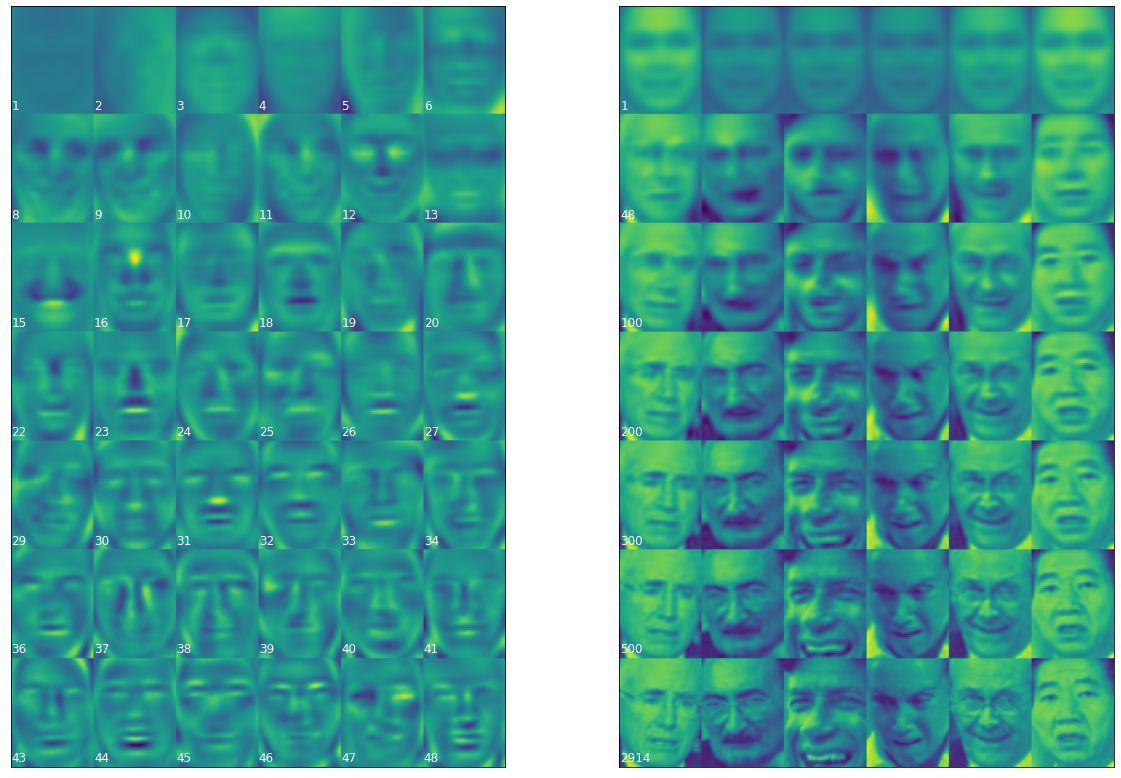
\includegraphics[width=\textwidth]{svd_eigenfaces.png}
    \caption{Left: The first 48 eigenfaces. The colorscale is consistent across the images. As can be expected, the eigenfaces seem to have an ordering from more general features, that are highly prevalent in the dataset, towards more specific features. Right: Five sample portraits from the dataset approximated using different numbers of eigenvectors. 2914 corresponds to the original image, which had 2914 pixels (degrees of freedom).}
    \label{fig:svd_eigenfaces}
\end{figure}

Facial recognition may be performed by projecting a new face into the space of eigenfaces and some form of matching to the coefficients of a known subject. This could be simply the euclidean distance, or it could be a classifier. In case of a classifier, the dimensionality reduction that is enabled by approximating images with a smaller set of eigenvectors may be critical to making the problem tractable by overcoming the curse of dimensionality.


% eigenbasis 
\subsection{Consistently Oriented Eigenbasis}
	
As discussed in section \ref{sec:svd}, the sign of the basis vectors can be flipped without affecting the validity of the singular value decomposition. That means that if the SVD is performed repeatedly on a slowly evolving system, the derived eigenbasis may abruptly change, for example, from a left-handed to a right-handed coordinate system. Hence there is a need to find a way to consistently orient the basis of eigenvectors. A heuristic technique consists of matching the eigenvectors that were derived from two separate decompositions by looking at their dot product, and flipping the signs in order to match them up. A more fundamentally rigorous technique was derived by \citeasnoun{damask2019consistently}. 


\section{Principal Component Analysis (PCA)}

Principal Component Analysis (PCA) is a decomposition of data into linearly uncorrelated components. It turns out that these axes are the right-singular eigenvectors $\mathbf{V}$ that are found from SVD. SVD and PCA have close correspondence (cf. section \ref{sec:pcasvd}).
\\

More elaborately, for a data matrix $\mathbf{X}\in\mathbb{R}^{N\times p}$, PCA extracts the ordered, rank-$p$, orthonormal basis in which the $p\times p$ covariance matrix of $\mathbf{X}$ is diagonal. The basis vectors are called the principal axes or principal directions of the data, and their ordering is by the magnitude of the variance that they explain. 
\\

The property that the covariance matrix is diagonal in the principal component basis means that projecting the data onto any of the basis vectors extracts a linearly uncorrelated component of the data that has variance corresponding to the corresponding eigenvalue of the covariance matrix.
\\

Just like with SVD, the ordering of the principal component basis in terms of their explained variance allows for lower-rank approximations of the data matrix to be constructed (section \ref{sec:svd}). Just like SVD, the lower rank approximations $\mathbf{X}$ are the best possible approximations with respect to the Frobenius Norm (cf. section \ref{sec:frobenius}). 
\\

The $p\times p$ covariance matrix  $\mathbf{C}$ of $\mathbf{X}$ is:

\begin{equation}
\mathbf{C} = \frac{\left(\mathbf{X}-\left<\mathbf{X}\right>\right)^T\left(\mathbf{X}-\left< \mathbf{X}\right>\right)}{n-1}
\end{equation}

Where $\left(\mathbf{X}-\left<\mathbf{X}\right>\right)^T$ is often referred to as the \textit{centered} data matrix. The covariance matrix is a symmetric, positive-definite matrix that can be diagonalized with orthonormal eigenvectors $\mathbf{V}$ and positive (or vanishing) eigenvalues $\lambda_i$:

\begin{equation}
\mathbf{C} = \mathbf{V}\mathbf{\Lambda}\mathbf{V}^T
\end{equation}

Where the eigenvectors in $V$ are ordered so that the eigenvectors along the diagonal of $\mathbf{\Lambda}$ have decreasing magnitude. The eigenvectors are the principal axes or principal directions of the data.




\subsection{Relationship between PCA and SVD}
\label{sec:pcasvd}
This is based on a great Stack Exchange answer \cite{amoeba2015svdpca}.

Let the singular value decomposition of the centered data matrix be:

\begin{equation}
\left(\mathbf{X}-\left<\mathbf{X}\right>\right) = \mathbf{U}\mathbf{\Sigma}\mathbf{V}^T
\end{equation}

Then:

\begin{equation}
\mathbf{C} = \frac{\mathbf{V\Sigma U}^T\mathbf{U\Sigma V}^T}{n-1} = \mathbf{V}\frac{\Sigma^2}{n-1}\mathbf{V}^T
\end{equation}

That means that:

\begin{itemize}
\item The principal axes are the right-singular vectors $\mathbf{V}$ that are obtained during SVD.
\item The singular values and the eigenvalues of the covariance matrix are related via $\lambda_i = \frac{\sigma_i^2}{n-1}$.
\end{itemize}


\section{$\mathbf{X}=\mathbf{W}\mathbf{H}$ Non-Negative Matrix Factorization}

Non-Negative Matrix Factorization works for positive matrices and is interesting as a method for dimensionality reduction. It works by expressing a matrix $\mathbf{X}\in\mathbb{R}^{p\times n}_+$ in terms of two smaller positive matrices $\mathbf{W}\in\mathbb{R}_+^{p\times r}$ and $\mathbf{H}\in \mathbb{R}^{r\times n}_+$. An excellent introduction is in \possessivecite{morningpaper2019nnmf} blog post and in \citeasnoun{gillis2014and}. 

Dimensionality reduction derives from the ability to adjust the rank of the decomposition via the dimension $r$.


\chapauthor{}	